\section{Results}

\subsection{Analysis}

I have tried multiple approaches to choose different hyper-parameters and model architecture. A few of the possible analyses are displayed below.

\subsubsection{Unidirectional LSTM}
As previously mentioned, I tried using unidirectional LSTM, but as part-of-speech tags depend on both the previous and following words in English, we moved to bi-directional LSTM. When Uni-directional LSTM was applied, the model functioned as shown below

\begin{figure}[h]
	\subfloat[Validation Set Accuracy]{{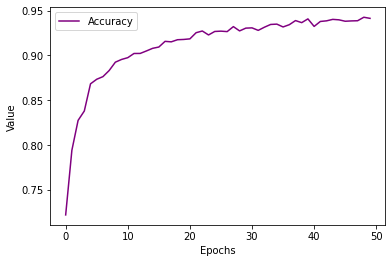
\includegraphics[scale=0.6]{img/6464ly2pt5uni/valid_acc.png} }}
    \subfloat[Validation Set Loss]{{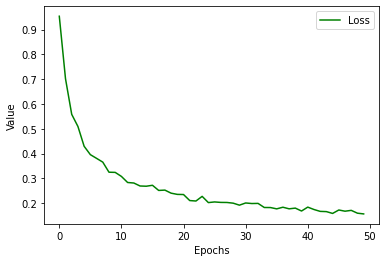
\includegraphics[scale=0.6]{img/6464ly2pt5uni/valid_loss.png}}}
    \caption{Validation Set Metrics on Uni-LSTM}
\end{figure}

\begin{figure}[h!]
	\centering
	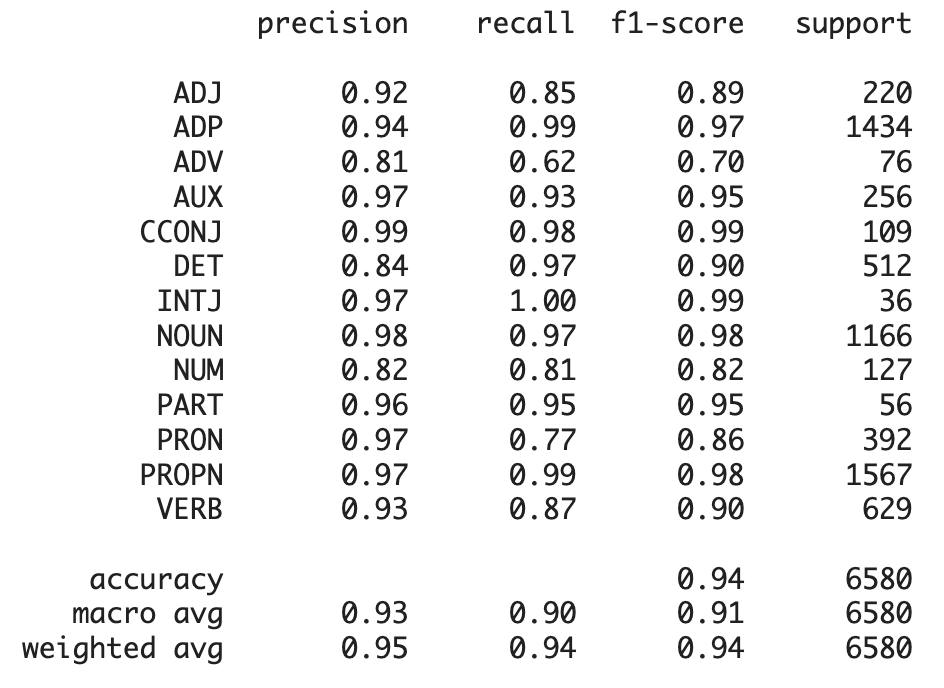
\includegraphics[scale=0.7]{img/unidirectionallstm.png}
	\caption{Classification Report for Uni-LSTM}
\end{figure}


\subsubsection{Hyper-parameters Tuning}

I adhered to the setting of the random search hyper-parameters method. For the Hidden Layer and Embedding Layer, I selected a set of values. I experimented with several different layers. These are some of the visual analyitcs

\begin{lstlisting}[language=Python]
	WORD_EMBEDDING_DIM = 32
	WORD_HIDDEN_DIM = 32
	EPOCHS = 50
	BIDIRECTIONAL = True
	DROPOUT = 0.5
	LEARNING_RATE = 0.005
	NUM_LAYERS = 2
\end{lstlisting}

\begin{figure}[h]
	\subfloat[Validation Set Accuracy]{{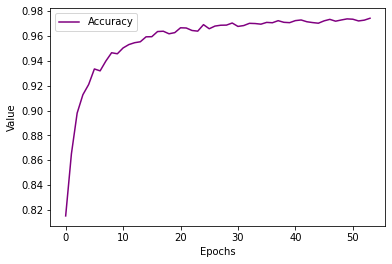
\includegraphics[scale=0.6]{img/3232pt5/valid_acc.png} }}
    \subfloat[Validation Set Loss]{{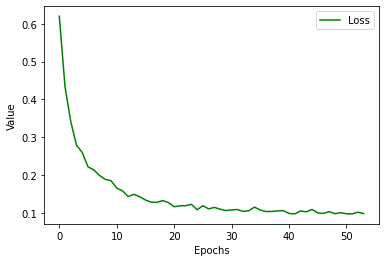
\includegraphics[scale=0.6]{img/3232pt5/valid_loss.png}}}
    \caption{Validation Set Metrics on various parameters}
\end{figure}


\begin{lstlisting}[language=Python]
	WORD_EMBEDDING_DIM = 64
	WORD_HIDDEN_DIM = 64
	EPOCHS = 50
	BIDIRECTIONAL = True
	DROPOUT = 0.5
	LEARNING_RATE = 0.005
	NUM_LAYERS = 3
\end{lstlisting}

\begin{figure}[h]
	\subfloat[Validation Set Accuracy]{{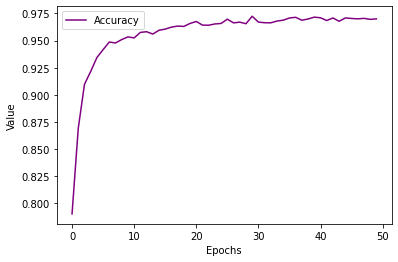
\includegraphics[scale=0.6]{img/6464ly3pt5/valid_acc.png} }}
    \subfloat[Validation Set Loss]{{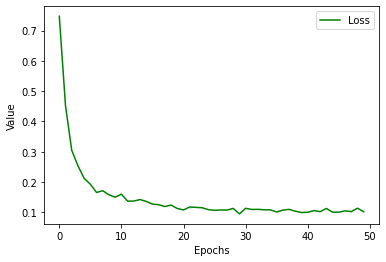
\includegraphics[scale=0.6]{img/6464ly3pt5/valid_loss.png}}}
    \caption{Validation Set Metrics on various parameters}
\end{figure}


\begin{lstlisting}[language=Python]
	WORD_EMBEDDING_DIM = 16
	WORD_HIDDEN_DIM = 16
	EPOCHS = 50
	BIDIRECTIONAL = True
	DROPOUT = 0.65
	LEARNING_RATE = 0.005
	NUM_LAYERS = 2
\end{lstlisting}

\begin{figure}[h]
	\subfloat[Validation Set Accuracy]{{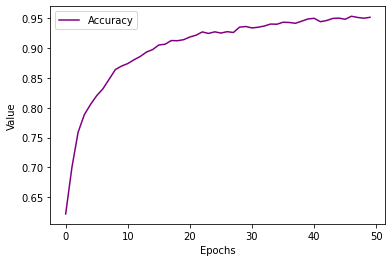
\includegraphics[scale=0.6]{img/1616pt65/valid_acc.png} }}
    \subfloat[Validation Set Loss]{{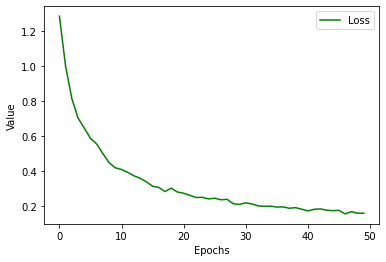
\includegraphics[scale=0.6]{img/1616pt65/valid_loss.png}}}
    \caption{Validation Set Metrics on various parameters}
\end{figure}




\subsection{Results}

After following the approach discussed above, I was able to achieve \textbf{98\% accuracy on the test dataset}.

Below is the \textit{classfication report} of the trained model

\begin{figure}[h]
	\centering
	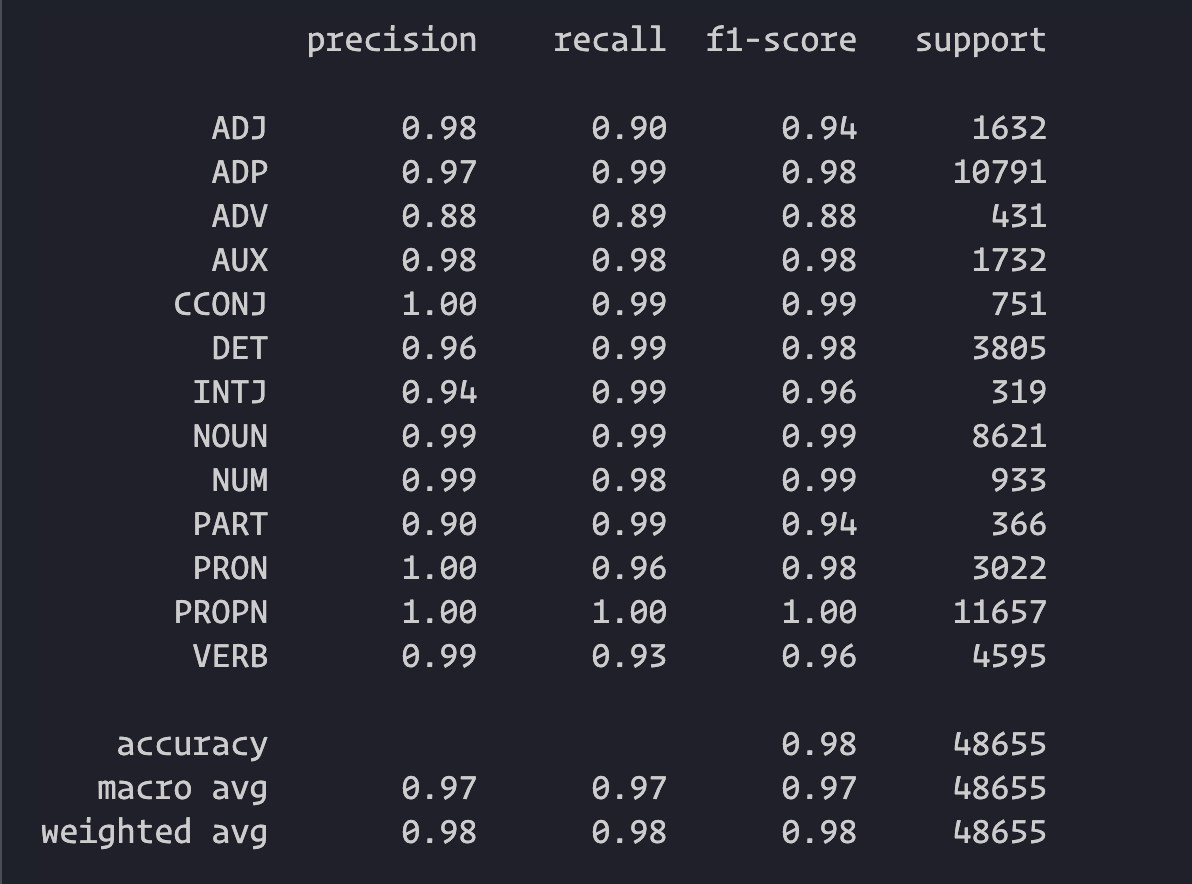
\includegraphics[scale=0.56]{img/class_report.png}
	\caption{Classification Report}
\end{figure}

The figures above depict various metrics such as \textit{precision, recall, and F1-score}, which provide a balance between precision and recall by computing their harmonic mean.


The below plots display the validation accuracy, as well as the loss during the training process. These plots provide an analysis of the model's performance with each epoch during training.

\begin{figure}[h]
	\subfloat[Validation Set Accuracy]{{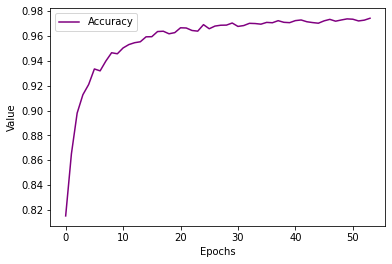
\includegraphics[scale=0.6]{img/3232pt5/valid_acc.png} }}
    \subfloat[Validation Set Loss]{{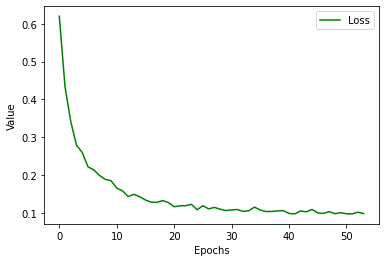
\includegraphics[scale=0.6]{img/3232pt5/valid_loss.png}}}
    \caption{Validation Set Metrics}
\end{figure}


The results demonstrate that as the number of epochs increase, there is a reduction in overall loss and an increase in accuracy. This indicates that the model has been effectively trained.   

\newpage

\subsection{Sample sentences test}

Below are some sample sentences to check how our model is predicting.

\begin{figure}[h]
	\centering
	\subfloat{{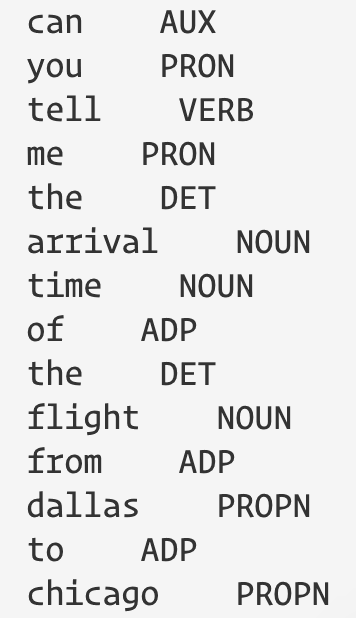
\includegraphics[scale=0.7]{img/sampleimg/sample1.png} }}
	\subfloat{{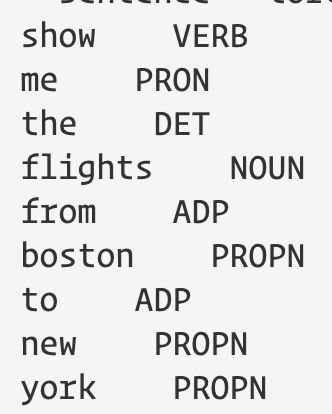
\includegraphics{img/sampleimg/sample2.png} }}
	\subfloat{{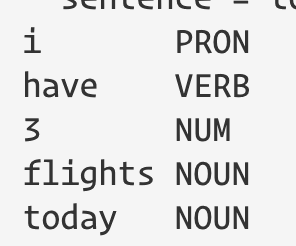
\includegraphics{img/sampleimg/sample3.png} }}
	\caption{Sample Sentences}
\end{figure}

